% Chapter where we present the results.

\chapter{Results}

In Chapter \ref{ch:methods} we discussed a general solution to the protoboard
layout problem, and various alternatives that can be used in implementing the
solution. Figure \ref{fig:alternatives} presents the alternatives in a structured
way. Here, we will explore these alternatives and compare them quantitatively.
This section will provide data that is useful in comparing the alternatives, and
the data will be discussed in detail in Chapter \ref{ch:discussion}.

\begin{figure}[H]
\Tree [.{All Alternatives}
    [{Distance} {Block} ].Placement !\qsetw{4cm}
    [{AP}
     [I D ].{PN}
     [I D ].{PP} ].Wiring !\qsetw{4cm}
    [{Component} {Wire} ].Resistors !\qsetw{4cm}
    [$A*$ {Best First} ].Search ]
\label{fig:alternatives}
\caption{All possible alternatives to the algorithm.}
\end{figure}

The data to compare the alternatives is gathered as described in Chapter
\ref{ch:methods}. We run the algorithm on $4425$ randomly generated schematics
of varying complexities. The algorithm is run $10$ times on each schematic.

In comparing alternatives, there are $3$ items we will consider:
\begin{enumerate}
\item Which alternative is the most successful?
\item Which alternative, when successful, takes the least amount of time?
\item Which alternative, when successful, produces the best layouts?
\end{enumerate}

In comparing success time, we will look at CPU time spent on the wiring step, as
the placement step has much less variability. We will look at plots of circuit
complexity versus wiring times to do the comparisons. Our measure of complexity
of a circuit will be the number of pins in the circuit as discussed in Chapter
\ref{ch:methods} (TODO: this is currently not done, be sure to give a histogram
of numbers of pins in the circuits).

In comparing the goodness of layouts, we will compare numbers of wires, total
lengths of wires, and numbers of wire crosses.

\section{Comparing placement methods}

\begin{figure}
\begin{center}
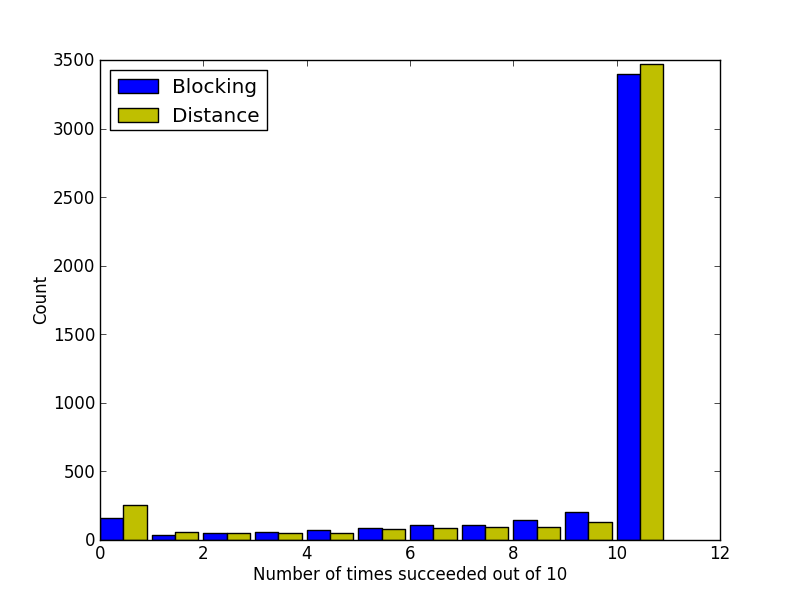
\includegraphics[width=\textwidth]{Images/placement_success_comparison.png}
\caption{TODO}
\label{fig:placement_success}
\end{center}
\end{figure}

\begin{table}[H]
\begin{center}
\begin{singlespace}
\begin{tabular}{|c||c|c|c|c|c|c|c|c|c|c|c|}
\hline
 & \multicolumn{11}{|c|}{Number of times solved out of $10$} \\
\hline
 & 0 & 1 & 2 & 3 & 4 & 5 & 6 & 7 & 8 & 9 & 10 \\
\hline\hline
Blocking & $162$ & $38$ & $51$ & $57$ & $72$ & $85$ & $109$ & $106$ & $144$ & $203$ & $3398$ \\
 & $0.04$ & $0.01$ & $0.01$ & $0.01$ & $0.02$ & $0.02$ & $0.02$ & $0.02$ & $0.03$ & $0.05$ & $0.77$ \\
\hline
 Distance & $258$ & $55$ & $54$ & $50$ & $52$ & $77$ & $86$ & $97$ & $93$ & $130$ & $3473$ \\
  & $0.06$ & $0.01$ & $0.01$ & $0.01$ & $0.01$ & $0.02$ & $0.02$ & $0.02$ & $0.02$ & $0.03$ & $0.78$ \\
\hline
\end{tabular}
\end{singlespace}
\end{center}
\caption{TODO}
\end{table}

\begin{figure}
\begin{center}
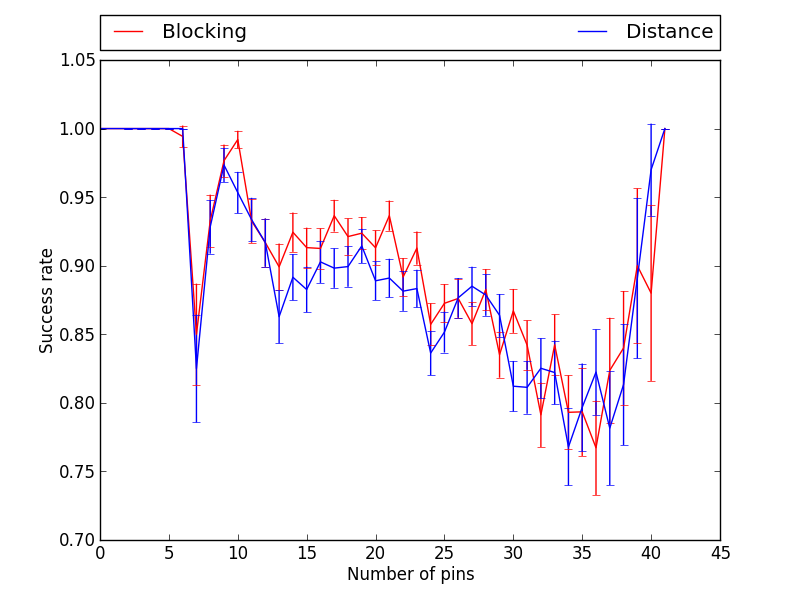
\includegraphics[width=\textwidth]{Images/placement_success_trend_comparison.png}
\caption{TODO}
\label{fig:placement_success_trend}
\end{center}
\end{figure}

\begin{figure}
\begin{center}
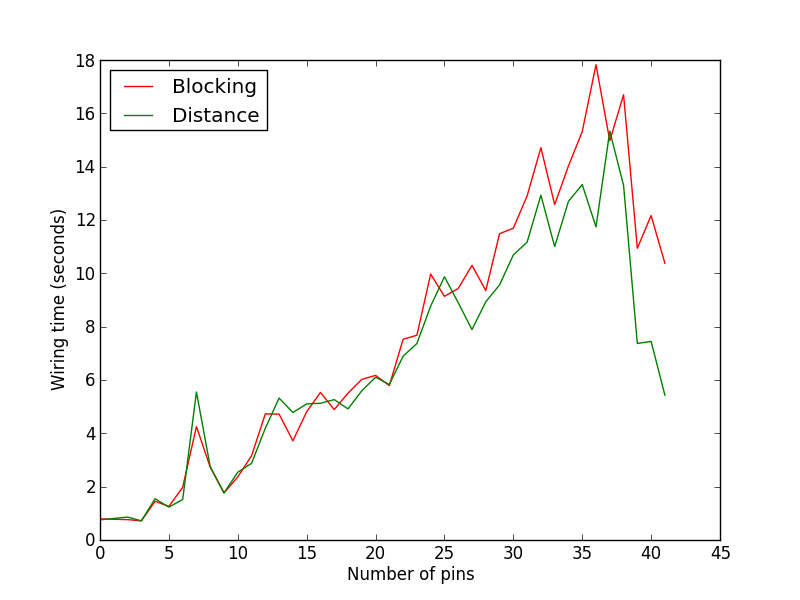
\includegraphics[width=\textwidth]{Images/placement_time_trend_comparison.png}
\caption{TODO}
\label{fig:placement_time_trend}
\end{center}
\end{figure}

\section{Comparing wiring methods}

\section{Comparing resistor treatments}

\section{Comparing search methods}

\section{Putting them all together}

\section{Exemplars}
